\documentclass[conference]{IEEEtran}

\usepackage{graphicx}
\usepackage{booktabs}
\usepackage{amsmath}
\usepackage{cite}

\title{Pathway-Aware Machine Learning for Type 2 Diabetes Classification from Human Pancreatic Beta-Cell Transcriptomes}

\author{
\IEEEauthorblockN{Tharuniya Anpalakan}
\IEEEauthorblockA{
Department of Applied Sciences\\
Northumbria University\\
Newcastle upon Tyne, United Kingdom\\
w25070895@northumbria.ac.lk
}
}

\begin{document}

\maketitle

\begin{abstract}
This exploratory study investigates whether biologically informed pathway-level features can support classification of type 2 diabetes (T2D) from human pancreatic beta-cell transcriptomic profiles while substantially reducing feature dimensionality. Donor-level beta-cell pseudobulk expression profiles were analysed for 34 individuals from the GSE221156 cohort, comprising 17 non-diabetic and 17 T2D donors. Differential expression analysis identified 1,334 genes with adjusted $p<0.05$, including 670 genes upregulated and 664 downregulated in T2D. KEGG pathway scores were derived from normalized beta-cell expression and evaluated using logistic regression with repeated stratified cross-validation. The pathway model achieved a mean balanced accuracy of 0.798 and mean ROC AUC of 0.865 using 291 pathway features, compared with 0.879 balanced accuracy and 0.931 ROC AUC for a 17,408-gene baseline model. Chemistry alone performed near chance, and inclusion of chemistry covariates did not materially alter pathway or gene-level performance. Independent validation was performed using beta-cell pseudobulk profiles from the E-MTAB-5061 cohort containing six non-diabetic and four T2D donors. After harmonising pathway definitions across studies, 277 pathways were retained. The fixed pathway model achieved an external ROC AUC of 0.833, accuracy of 0.700, and balanced accuracy of 0.625. These results suggest that pathway-level representations retain substantial predictive information while greatly reducing feature dimensionality, although cross-study probability calibration remains limited.
\end{abstract}

\begin{IEEEkeywords}
type 2 diabetes, single-cell RNA sequencing, beta cells, pathway analysis, machine learning, transcriptomics, external validation
\end{IEEEkeywords}

\section{Introduction}

Type 2 diabetes mellitus (T2D) is a complex metabolic disorder involving impaired insulin secretion, insulin resistance, and progressive dysfunction of pancreatic beta cells. Transcriptomic profiling provides an opportunity to characterize molecular alterations associated with beta-cell dysfunction, as demonstrated by human pancreatic single-cell studies~\cite{muraro2016,baron2016,segerstolpe2016}; however, high-dimensional gene-expression measurements present challenges for robust statistical modelling, particularly when the number of measured genes greatly exceeds the number of available donors.

This study evaluates whether KEGG pathway-level features derived from human pancreatic beta-cell transcriptomes can discriminate between non-diabetic and T2D donors. The pathway model is compared with a high-dimensional gene-level baseline and a technical chemistry-only model. Predictive stability and potential chemistry confounding are evaluated, and the resulting pathway model is subsequently tested in an independent human pancreatic single-cell dataset.

\section{Methods}

\subsection{Discovery Cohort and Beta-Cell Pseudobulk Expression}

The discovery analysis used donor-level beta-cell pseudobulk expression profiles derived from the GSE221156 human pancreatic single-cell RNA-sequencing dataset described by Bandesh et al.~\cite{bandesh2026}. Only non-diabetic (ND) and T2D donors were retained, resulting in 34 donors: 17 ND and 17 T2D.

Genes were retained when they had a raw count of at least 10 in at least five donors. This filtering step retained 17,408 genes. Library-size normalization was performed using counts per million (CPM), followed by $\log_2(\mathrm{CPM}+1)$ transformation.

\subsection{Differential Expression Analysis}

Differential expression between T2D and ND donors was performed using DESeq2~\cite{love2014} on donor-level beta-cell pseudobulk counts. Genes with Benjamini--Hochberg adjusted $p<0.05$ were considered statistically significant.
Donor-level aggregation was used to reduce the risk of inflated significance arising from treating individual cells as independent biological replicates~\cite{squair2021}.
\subsection{Pathway Enrichment Analysis}

Significantly upregulated and downregulated genes were analysed using KEGG 2021 Human~\cite{kanehisa2000} and Gene Ontology Biological Process gene sets~\cite{go2021}, with enrichment implemented using GSEApy~\cite{fang2023}.

\subsection{Pathway Feature Construction}

KEGG 2021 Human gene sets were mapped to the 17,408 expressed genes in the discovery cohort. Pathways containing between 10 and 200 expressed genes were retained, resulting in 291 pathways.

For each donor and pathway, the pathway score was calculated as the mean $\log_2(\mathrm{CPM}+1)$ expression of genes belonging to that pathway.

\subsection{Machine-Learning Models}

Three primary logistic-regression models were evaluated:

\begin{enumerate}
    \item a pathway-level model using 291 KEGG pathway features;
    \item a gene-level model using 17,408 normalized gene-expression features; and
    \item a chemistry-only model using sequencing chemistry as the predictor.
\end{enumerate}

Features were standardized using a standard scaler within each modelling pipeline, with logistic regression and cross-validation implemented using scikit-learn~\cite{pedregosa2011}. Model performance was evaluated using repeated stratified five-fold cross-validation with 20 repeats. Accuracy, balanced accuracy, and receiver operating characteristic area under the curve (ROC AUC) were calculated.

Additional models combining biological features with chemistry were evaluated to assess whether sequencing chemistry accounted for predictive performance.

\subsection{External Validation}

Independent validation was performed using the E-MTAB-5061 human pancreatic single-cell dataset reported by Segerstolpe et al.~\cite{segerstolpe2016}. Metadata contained six non-diabetic donors and four donors with type II diabetes mellitus.
A total of 270 cells annotated as beta cells were identified. Raw beta-cell counts were aggregated to donor-level pseudobulk profiles. Duplicate gene symbols were collapsed by summing counts, followed by gene filtering, CPM normalization, and $\log_2(\mathrm{CPM}+1)$ transformation.

To avoid external-label leakage, pathway definitions were determined using the discovery cohort and then matched to genes measurable in both studies. Pathways containing at least 10 shared genes were retained, producing 277 matched KEGG pathways.

A logistic-regression model was trained exclusively on the 34 discovery donors using these matched pathway features and applied without retraining to the 10 independent external donors.

\section{Results}

\subsection{Differential Expression in T2D Beta Cells}

Differential-expression analysis identified 1,334 significant genes at adjusted $p<0.05$. Of these, 670 genes showed increased expression in T2D and 664 showed decreased expression.

Pathway enrichment among genes upregulated in T2D included neuroactive ligand--receptor interaction, ECM--receptor interaction, cytokine--cytokine receptor interaction, calcium-related signalling, synaptic signalling, and cAMP signalling. Downregulated genes showed enrichment for pathways including maturity onset diabetes of the young and carbohydrate digestion and absorption.

\subsection{Predictive Performance}

The pathway model achieved a mean repeated-cross-validation accuracy of 0.798, mean balanced accuracy of 0.798, and mean ROC AUC of 0.865.

The gene-level model achieved higher predictive performance, with a mean accuracy of 0.881, mean balanced accuracy of 0.879, and mean ROC AUC of 0.931.

The chemistry-only model performed substantially worse, with a mean balanced accuracy of 0.556 and mean ROC AUC of 0.578.

Despite its lower performance relative to the gene-level model, the pathway representation reduced the number of predictive features from 17,408 genes to 291 pathways, corresponding to an approximately 98.3\% reduction in dimensionality.

\begin{figure}[!t]
\centering
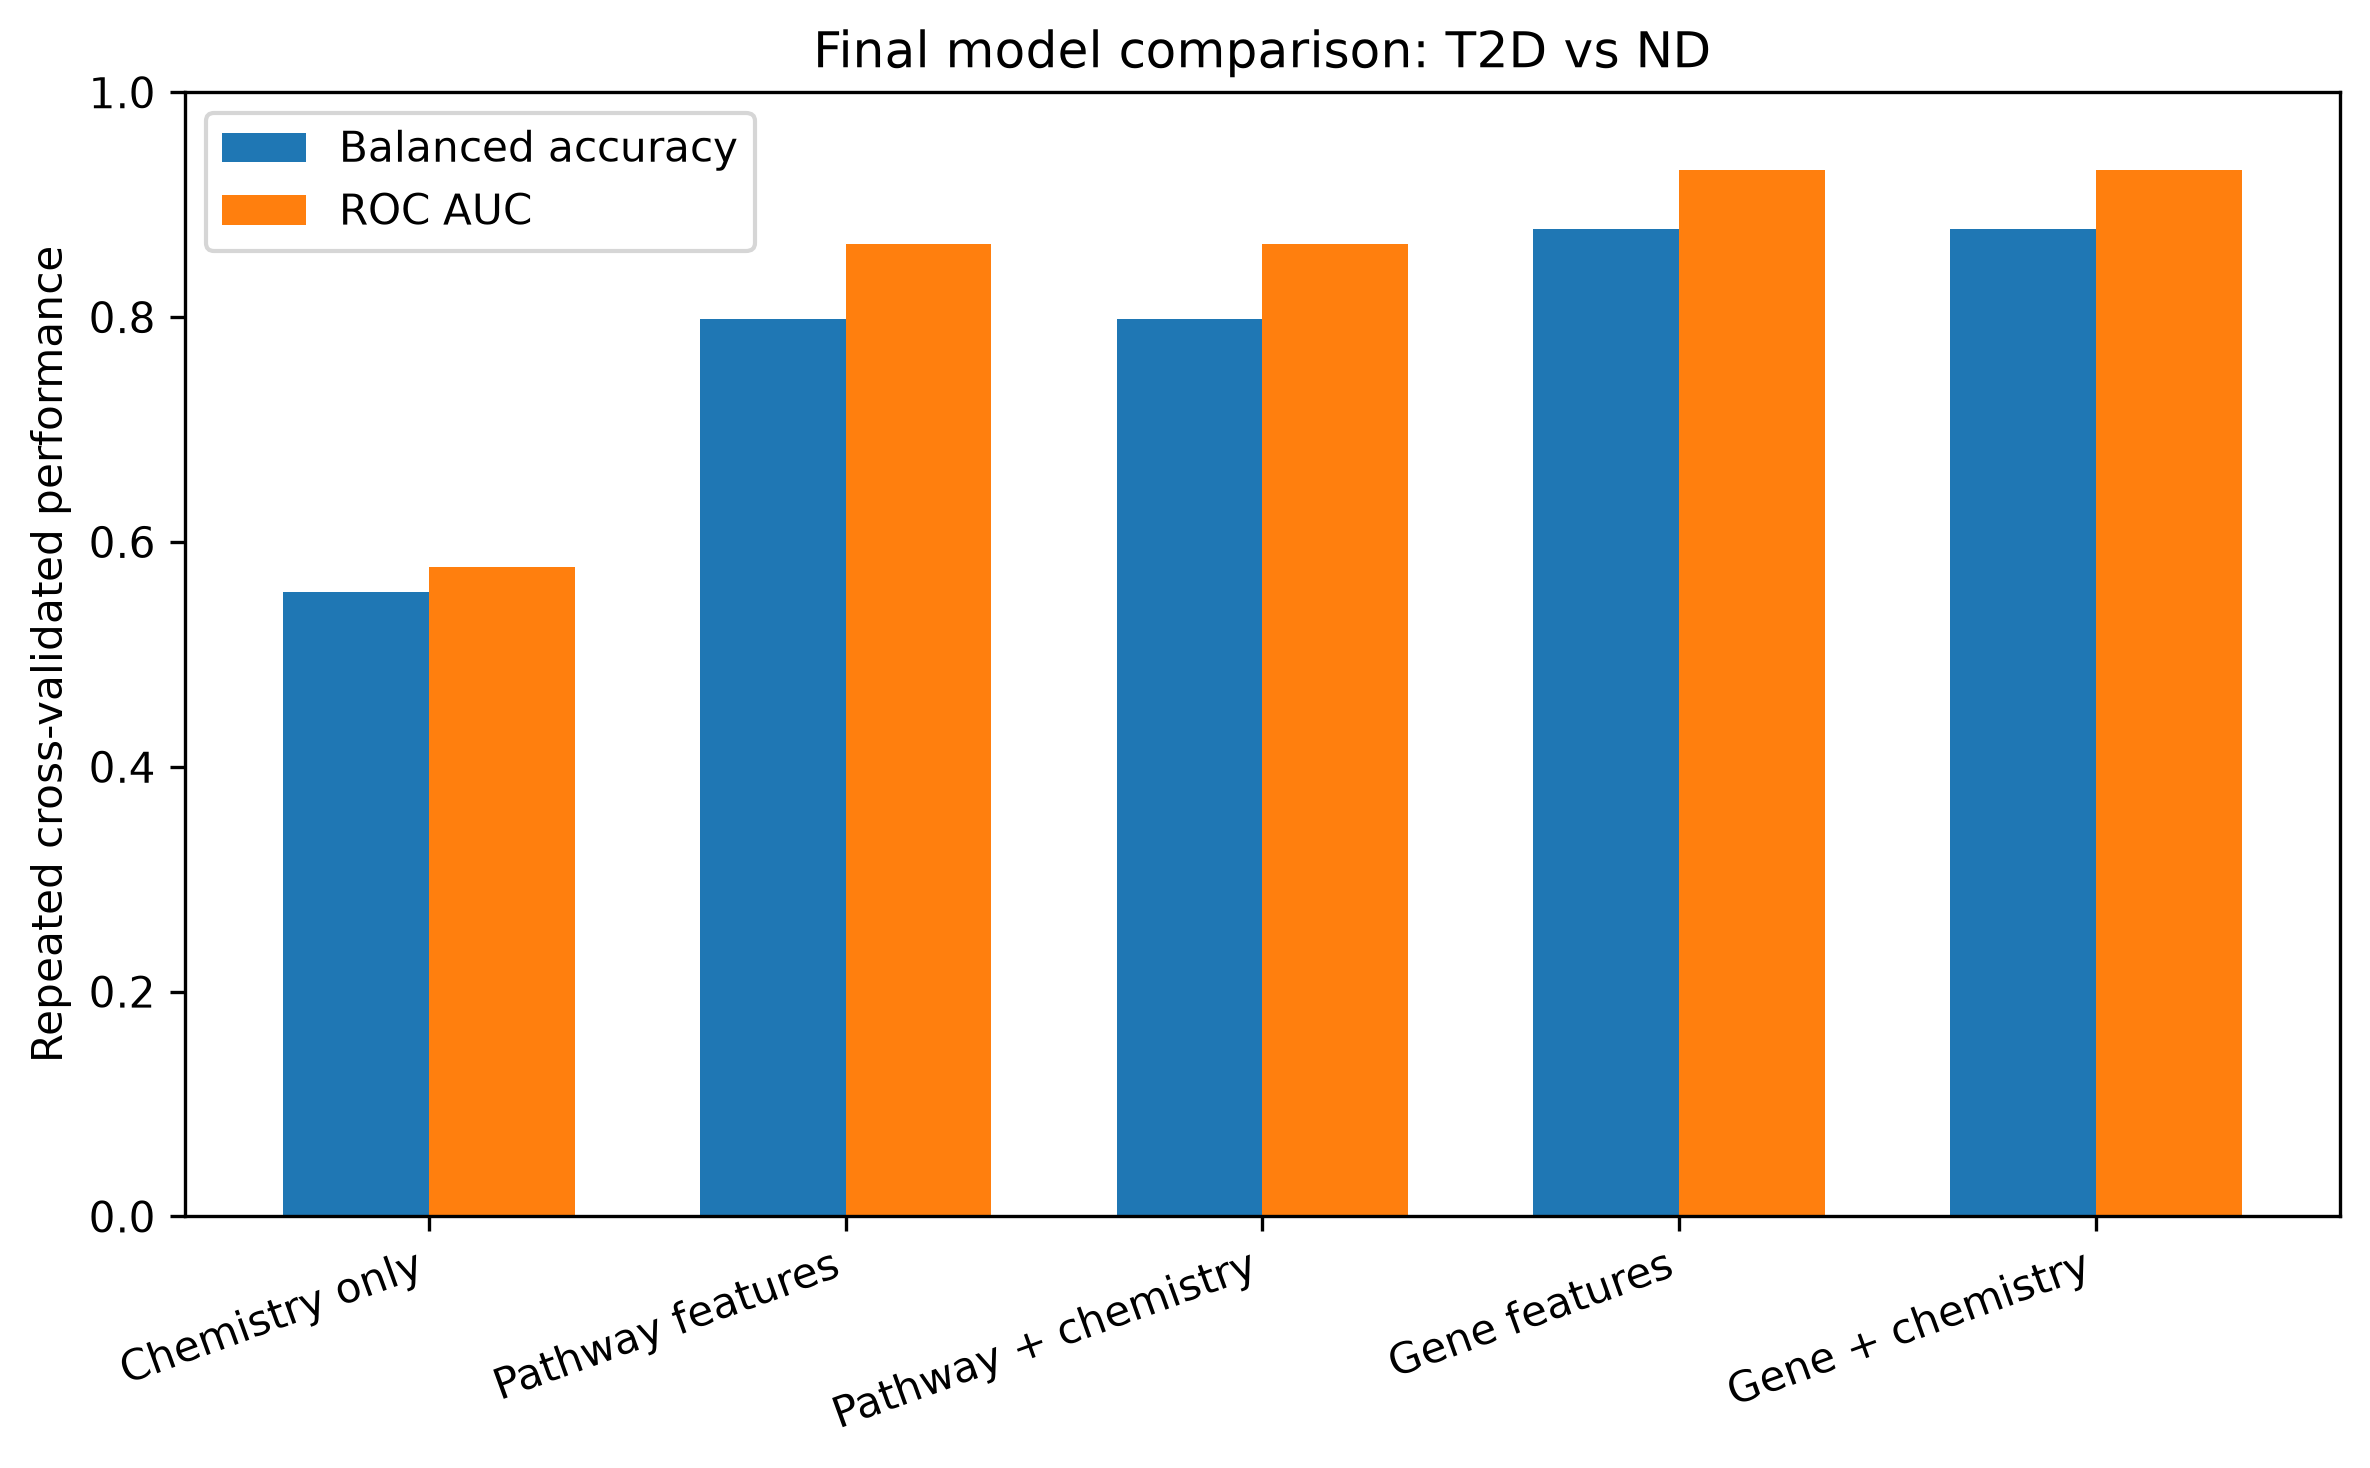
\includegraphics[width=\columnwidth]{../results/figures/final_model_comparison.png}
\caption{Comparison of predictive performance for chemistry-only, pathway, pathway-plus-chemistry, gene, and gene-plus-chemistry logistic-regression models.}
\label{fig:modelcomparison}
\end{figure}

\subsection{Stable Pathway Predictors}

Repeated cross-validation was used to assess coefficient stability across training folds. Several pathways showed consistent coefficient direction across all folds, including arginine biosynthesis, pentose and glucuronate interconversions, central carbon metabolism in cancer, carbohydrate digestion and absorption, maturity onset diabetes of the young, type I diabetes mellitus, arginine and proline metabolism, retinol metabolism, and thiamine metabolism.

Disease-named KEGG pathways should be interpreted as shared gene-expression programs rather than evidence that donors have the corresponding diseases.

\begin{figure}[!t]
\centering
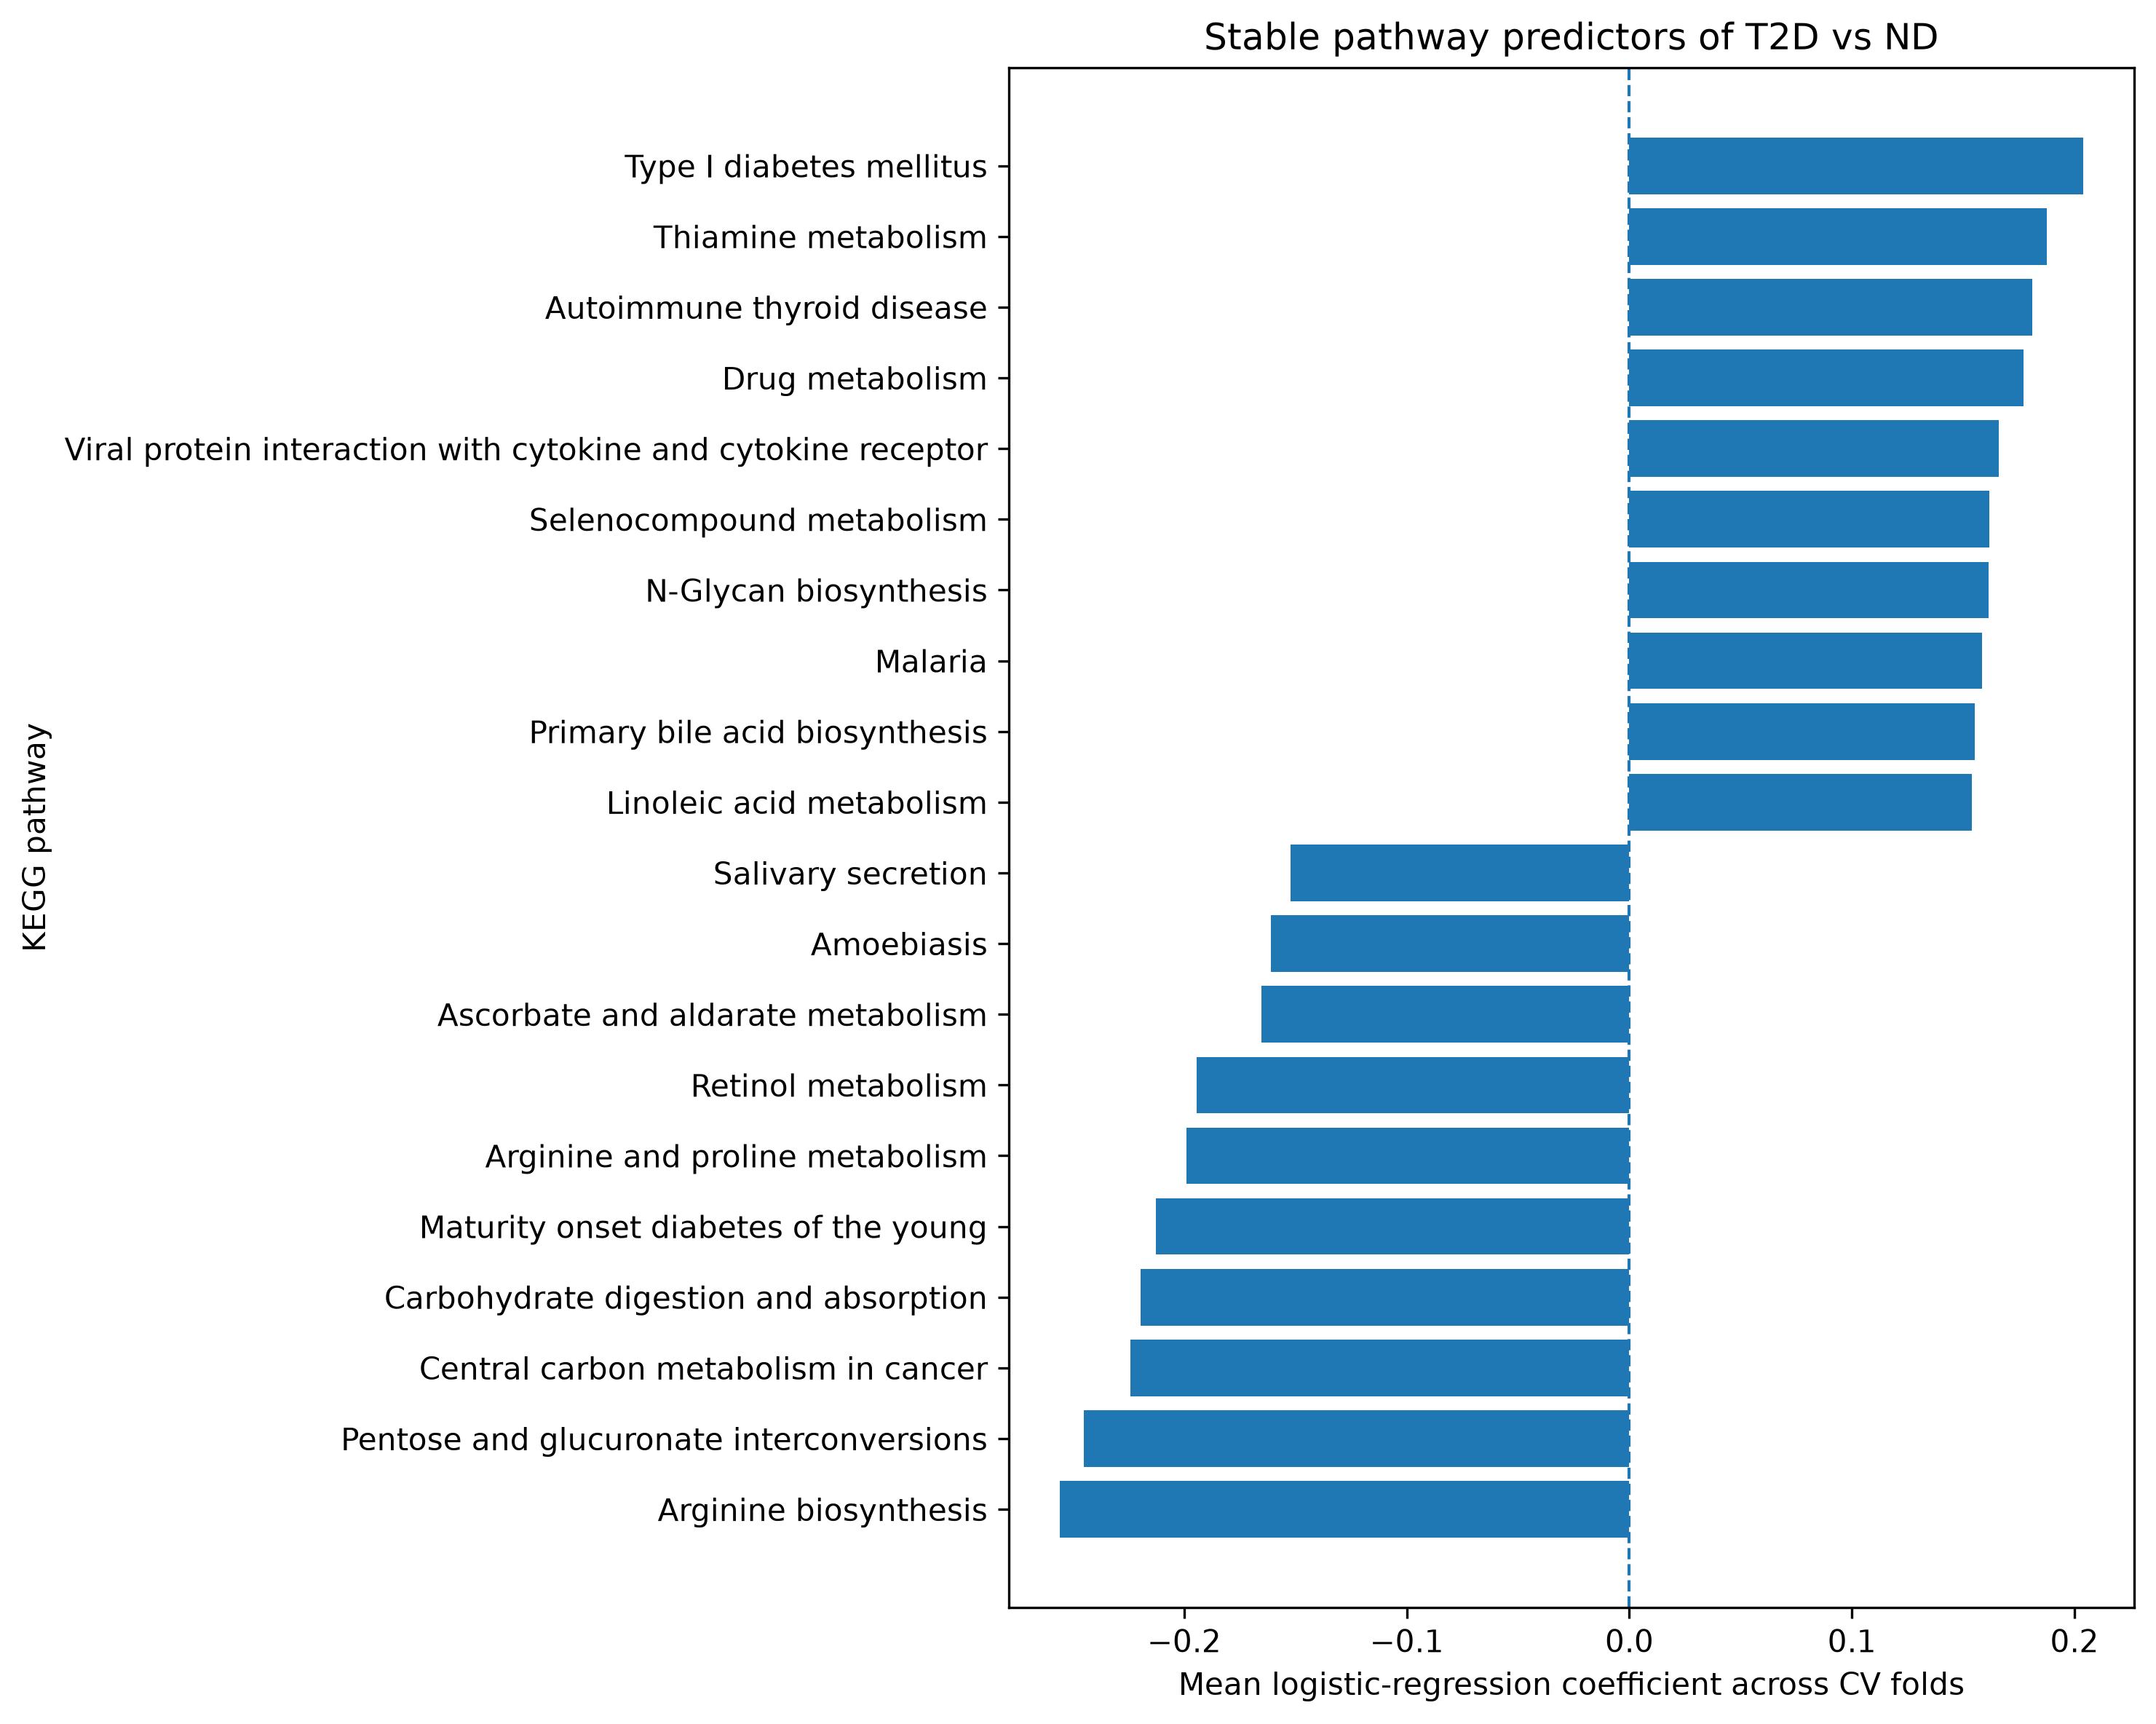
\includegraphics[width=\columnwidth]{../results/figures/stable_pathway_predictors.png}
\caption{Stable pathway predictors identified across repeated cross-validation folds.}
\label{fig:stablepathways}
\end{figure}

\subsection{Independent External Validation}

The independent E-MTAB-5061 validation cohort contained six ND and four T2D donors. Of the 291 discovery pathways, 277 retained at least 10 genes measurable in both datasets.

The pathway model trained exclusively on the discovery cohort achieved an external accuracy of 0.700, balanced accuracy of 0.625, and ROC AUC of 0.833.

All six ND donors were classified correctly using the default probability threshold of 0.5, whereas one of four T2D donors was classified as T2D. Despite this threshold-dependent performance, T2D donors generally received higher predicted T2D probabilities than ND donors, indicating preservation of cross-study ranking information.

\begin{figure}[!t]
\centering
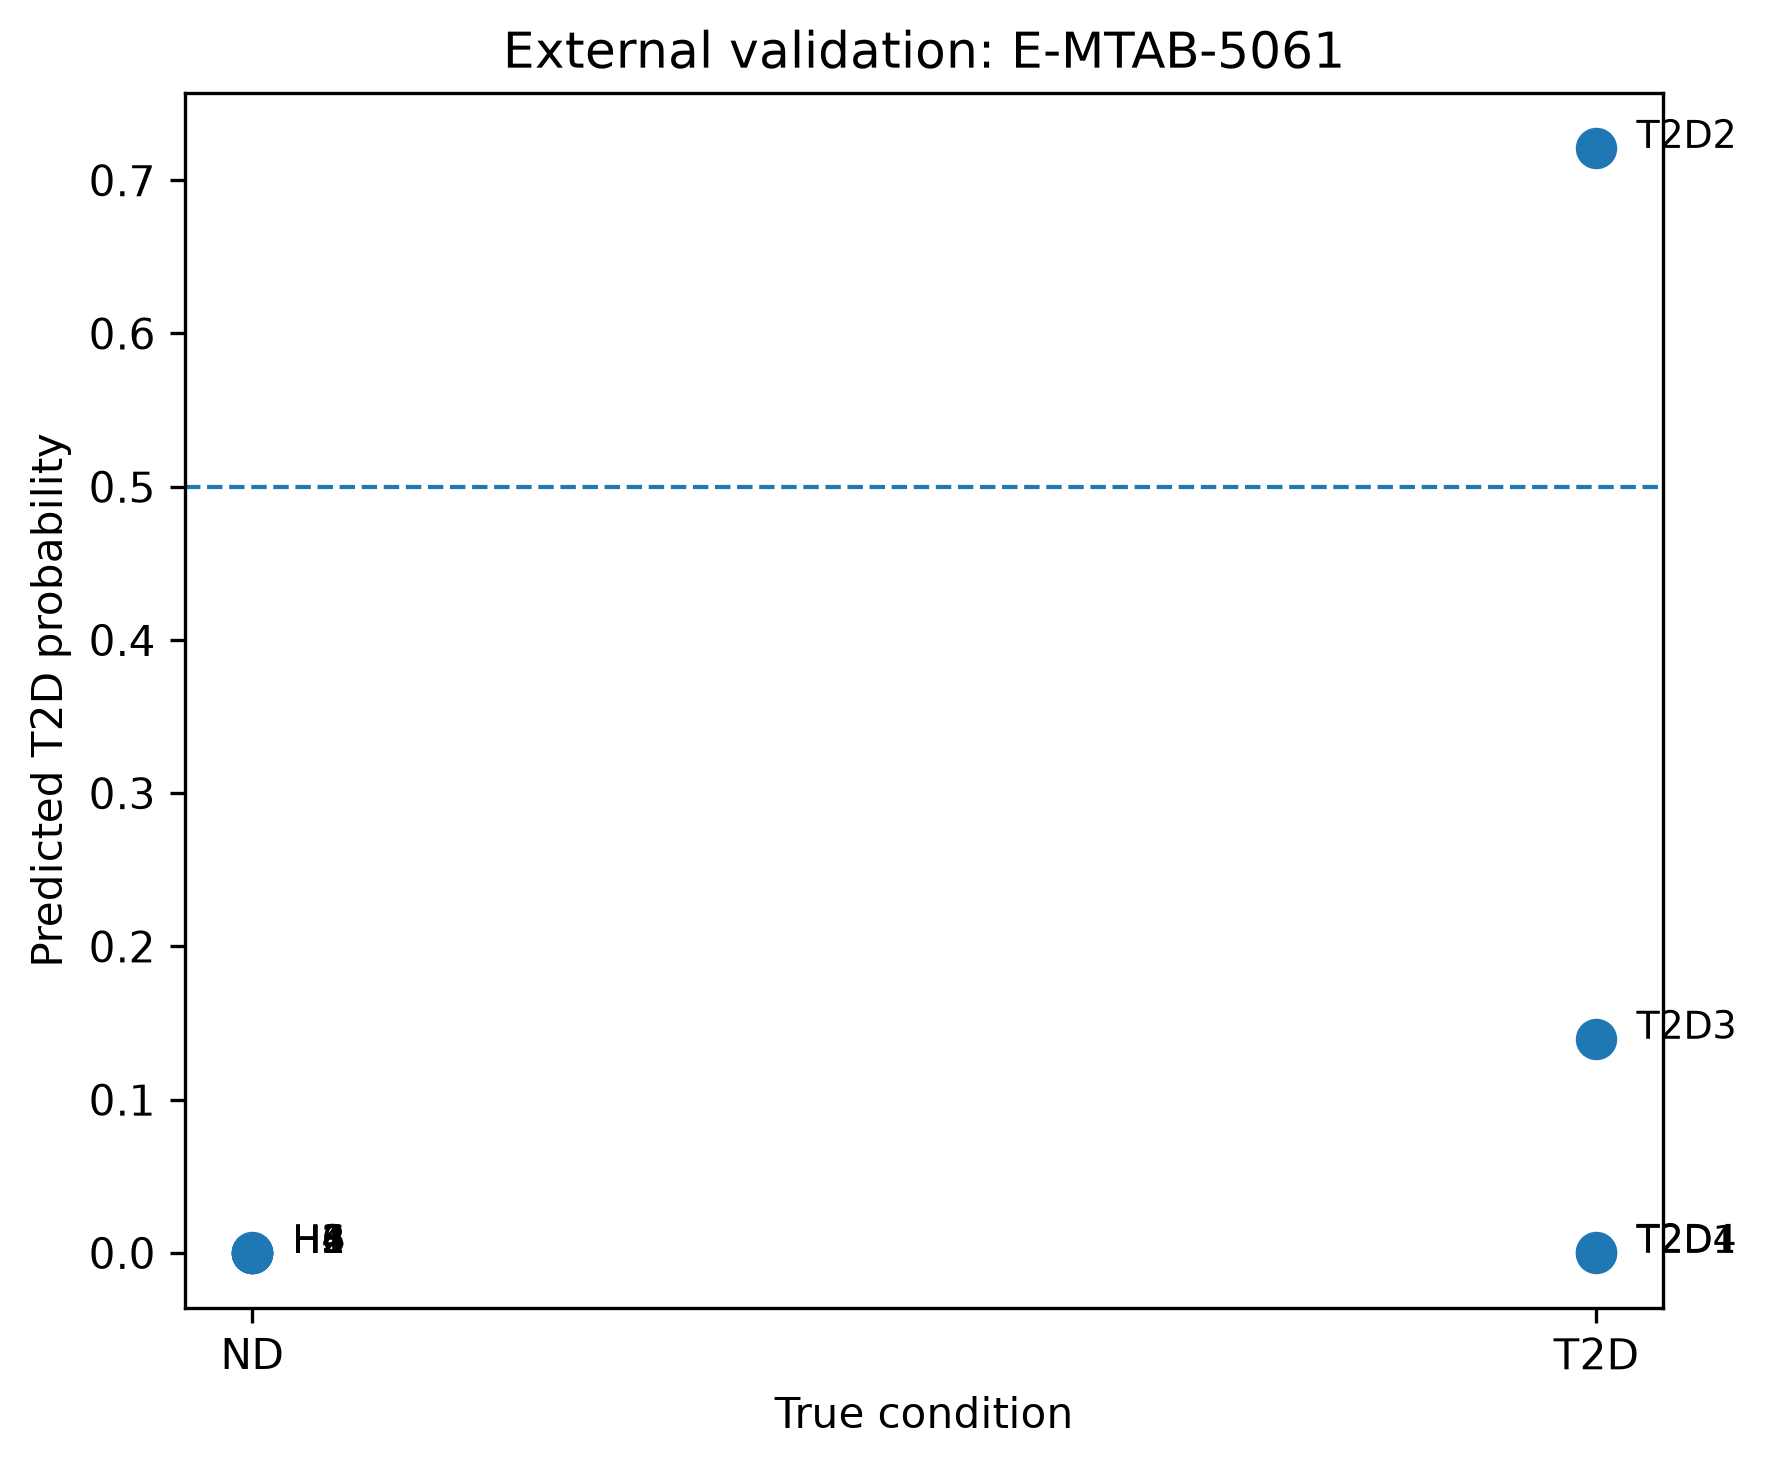
\includegraphics[width=\columnwidth]{../results/figures/external_validation_probabilities.png}
\caption{Predicted T2D probabilities for donors in the independent E-MTAB-5061 cohort. The dashed horizontal line indicates the default 0.5 classification threshold.}
\label{fig:externalvalidation}
\end{figure}

\section{Discussion}

This study demonstrates that pathway-level transcriptomic features retain substantial information for distinguishing T2D from non-diabetic pancreatic beta-cell profiles while substantially reducing feature dimensionality.

The gene-level model produced the strongest internal predictive performance. Therefore, the results do not support the conclusion that pathway features outperform individual-gene features. Instead, the pathway representation offers a trade-off between predictive performance, interpretability, and dimensionality reduction.

The chemistry-only model performed near chance, and addition of chemistry to pathway and gene-expression models did not materially improve predictive performance. These findings suggest that sequencing chemistry was not the principal source of the observed disease discrimination.

Independent validation provided further evidence that pathway-derived signals generalize across datasets. The external ROC AUC of 0.833 indicates useful ranking discrimination. However, the majority of external predicted probabilities were shifted below the default 0.5 threshold, resulting in lower balanced accuracy. This behaviour is consistent with cross-study distribution and calibration differences arising from independent cohorts, sequencing protocols, and data-processing pipelines.

The external cohort contained only 10 donors, including four T2D cases. Consequently, the external performance estimates are uncertain and should be interpreted as supportive rather than definitive validation.

Additional limitations include the modest discovery-cohort size, reliance on predefined pathway databases, and potential biological heterogeneity between donors. Larger independent cohorts will be required to assess reproducibility and calibration more precisely.

\section{Conclusion}

Pathway-aware modelling of pancreatic beta-cell transcriptomes provides a compact and biologically interpretable representation of T2D-associated molecular variation. Although a high-dimensional gene-level model achieved higher internal predictive performance, the pathway model retained strong discrimination using approximately 98\% fewer features and achieved an external ROC AUC of 0.833 in an independent cohort. These findings support further investigation of pathway-level representations for interpretable transcriptomic classification and cross-study validation in diabetes research.

\bibliographystyle{IEEEtran}
\bibliography{references}

\end{document}